\documentclass[oneside,11pt,a4paper]{article}

% PACKAGES %

\usepackage[utf8]{inputenc}    
\usepackage[T1]{fontenc}
\usepackage[english]{babel}
\usepackage{graphicx}
\usepackage{layout}
\usepackage{color}
\usepackage{lipsum}
\usepackage{tikz}
\usepackage{lscape}
\usepackage{listings}
\usepackage{amsmath}
\usepackage{amssymb}
\usepackage{placeins}
\usepackage{array}
\usepackage{hyperref}
\usepackage{enumerate}
%\usepackage[active,tightpage]{preview}

% D�fini les marges � 2 cm
\usepackage[top=1cm, bottom=2cm, left=2.5cm, right=2.5cm]{geometry}

% Supprime l'indentation de la premi�re ligne des paragraphes
\setlength{\parindent}{0pt}
\setlength{\parskip}{10pt}

\addto\captionsenglish{% Replace "english" with the language you use
  \renewcommand{\contentsname}%
    {Table of contents}%
}

\definecolor{keywordsColor}{rgb}{0,0.5,0}

\lstset{ %
  backgroundcolor=\color{white},   % choose the background color; you must add \usepackage{color} or \usepackage{xcolor}
  basicstyle=\footnotesize\ttfamily,        % the size of the fonts that are used for the code
  breakatwhitespace=false,         % sets if automatic breaks should only happen at whitespace
  breaklines=true,                 % sets automatic line breaking
  captionpos=none,                    % sets the caption-position to none
  columns=fixed,
  commentstyle=\color{green},    % comment style
  escapeinside={\%*}{*)},          % if you want to add LaTeX within your code
  extendedchars=true,              % lets you use non-ASCII characters; for 8-bits encodings only, does not work with UTF-8
 % frame=single,                    % adds a frame around the code
  keywordstyle=\bfseries\color{keywordsColor},       % keyword style
  language=SQL,                 % the language of the code
  numbers=left,                    % where to put the line-numbers; possible values are (none, left, right)
  numbersep=10pt,                   % how far the line-numbers are from the code
  numberstyle=\tiny\color{gray}, % the style that is used for the line-numbers
  morekeywords={REFERENCES},
  deletekeywords={YEAR},
  rulecolor=\color{black},         % if not set, the frame-color may be changed on line-breaks within not-black text (e.g. comments (green here))
  showspaces=false,                % show spaces everywhere adding particular underscores; it overrides 'showstringspaces'
  showstringspaces=false,          % underline spaces within strings only
  showtabs=false,                  % show tabs within strings adding particular underscores
  stepnumber=1,                    % the step between two line-numbers. If it's 1, each line will be numbered
  stringstyle=\color{blue},     % string literal style
  tabsize=2,                       % sets default tabsize to 2 spaces
  title=\lstname                   % show the filename of files included with \lstinputlisting; also try caption instead of title
}

% DOCUMENT %

\begin{document}
\title{Database project - deliverable 3}
\author{
	Arthur \sc{Giroux}\\\small{205443}
	\and
	Colla \sc{Rensch}\\\small{205814}
	\and
	Valentin \sc{Matter}\\\small{203447}
}
\date{June $2^{\textrm{nd}}$ 2013} 

\maketitle

\tableofcontents
\vskip 170pt
Our web front-end is available at \url{http://db.tamere.ch/}
\\\\Access is made using the password : \textbf{dias2013}

\part*{Deliverable 1}
\addcontentsline{toc}{section}{Deliverable 1}

\section*{ER model}
\addcontentsline{toc}{subsection}{ER model}

\begin{center}
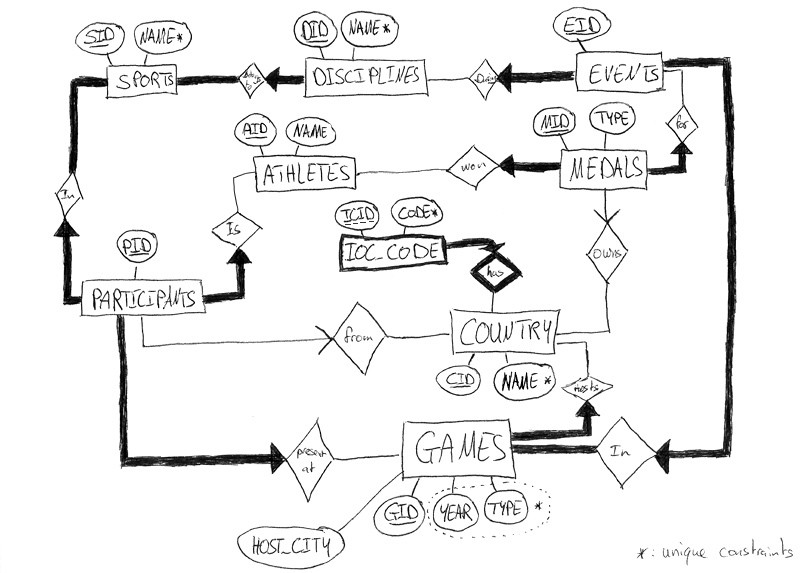
\includegraphics[height=310px]{images/ermodel.jpg}
\end{center}

\section*{Tables creation}
\addcontentsline{toc}{subsection}{Tables creation}

\lstinputlisting{db.sql}

\section*{Remarks}
\addcontentsline{toc}{subsection}{Remarks}

\begin{itemize}
	\item Athletes is the entity that stores the information of an athlete who can then participate in multiple sports or games. Which means that if an Athlete competes twice he will have only one entry in the ATHLETES table but two in the PARTICIPANTS table.
	\item Each game should at least have one event otherwise nothing happened during he games. The same applies to sports, a sport must have at least one participant, otherwise the sport never took place during any games.
	\item Countries, sports and disciplines must have a unique name as the opposite would have no sense. For games it is the pair (YEAR,TYPE) that must be unique.
	\item Due to problem with their federations some athletes may present themselves without representing a country.
	\item Some medals could not be associated to a country as some athletes aren't as for the above point.
	\item The numbers of countries, athletes and events for a given game isn't stored in the GAMES entity as they can be easily computed using some COUNT query.
	\item The names of the events, disciplines and games are not stored as they are only the concatenation of information stored in other tables.
\end{itemize}

\part*{Deliverable 2}
\addcontentsline{toc}{section}{Deliverable 2}

\section*{Modifications}
\addcontentsline{toc}{subsection}{Modifications}

We had to slightly modify our model as we forced each athlete to have a binding participant, but we noticed that there is a quite big amount of them that do not. Therefore, we decided to slightly change our ER-model as to allow athletes to not have a binding participant. No change to the table creation code was needed as it is not possible to represent the "at least" constraint.

\section*{Data import}
\addcontentsline{toc}{subsection}{Data import}

We chose to import the data using Java. We decided that any data that would generate a non-existent foreign key would be dropped as would any inconsistent or incomplete data (i.e. medals without color)

\part*{Deliverable 3}
\addcontentsline{toc}{section}{Deliverable 3}

\section*{Modifications and Design choices}
\addcontentsline{toc}{subsection}{Modifications}

\begin{enumerate}
	\item To allow us a good way to differentiate individuals from teams we added a team ID attribute "TID" to the medals. TID would be NULL is the medal belongs to an individual and would not be NULL if it belonged to a team (all medals of a team have the same TID)
	\item We encountered a problem when setting up our deleting interface, we didn't use cascades at all. We changed it in a way that now all foreign key cascade on update and delete.
	\item Another thing we changed (added) is a view called Medals\_Unique (see below). It's a view of our Medals table where we have all the individual medals and one medal per team. Which is very useful when counting medals.
\begin{lstlisting}
CREATE VIEW MEDALS_UNIQUE AS (
  SELECT MIN(M.MID) AS MID, M.CID, M.TYPE, M.EID 
  FROM MEDALS M
  WHERE M.TID IS NOT NULL
  GROUP BY M.TID
) UNION (
  SELECT M.MID, M.CID, M.TYPE, M.EID 
  FROM MEDALS M
  WHERE M.TID IS NULL
)
\end{lstlisting}
\end{enumerate}

\section*{Performance}
\addcontentsline{toc}{subsection}{Performance}

After spending a very large amount of time on trying to add indexes that could improve the performance of our queries (we ran them over and over again using average time over 20, 50 or 100 executions and adding pretty much all possible indexes, we had to resign to the fact that adding indexes does not improve our queries. This is due to the fact that MySQL enforces indexes on foreign keys, unique keys and referenced keys so that foreign key checks can be fast and not require a table scan. Indeed the only indexes left would be GAMES TYPE and HOST\_CITY but given the small size of the GAMES table (52) an index would be useless, we then have the MEDALS TYPE and TID, the first is of no use as there is only 3 possible values for TYPE, the second is useless too, as most of the TIDs are NULL rendering an index on it pointless. Finally ATHELETE NAME which could be potentially useful as athlete is our biggest table however it is of no use for our queries.
Additionally our schema was made in such a way that we use almost all the time either a primary either a foreign key in our SQL statements. 

Thus, we were not able to make any query faster by adding an index as every queries are already using indexes.

\part*{Front-end}
\addcontentsline{toc}{section}{Front-end}

Our web front-end is available at \url{http://db.tamere.ch/}. It was made using PHP and MySQL.

\begin{center}
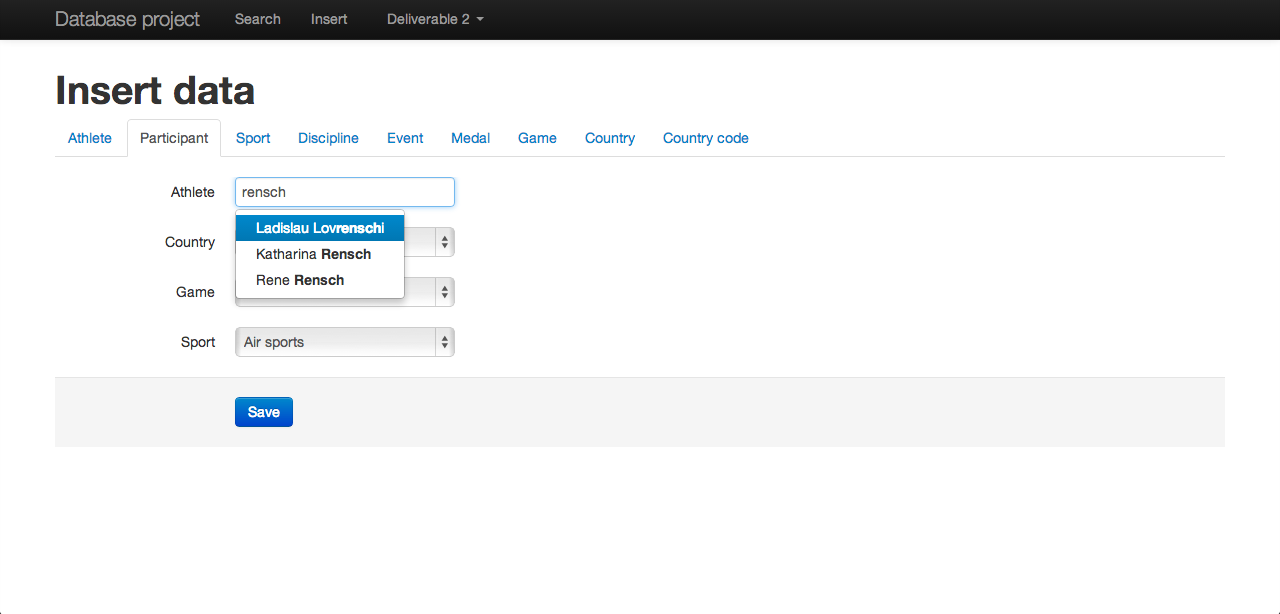
\includegraphics[height=210px]{images/capt1.png}
The insertion page
\end{center}

\begin{center}
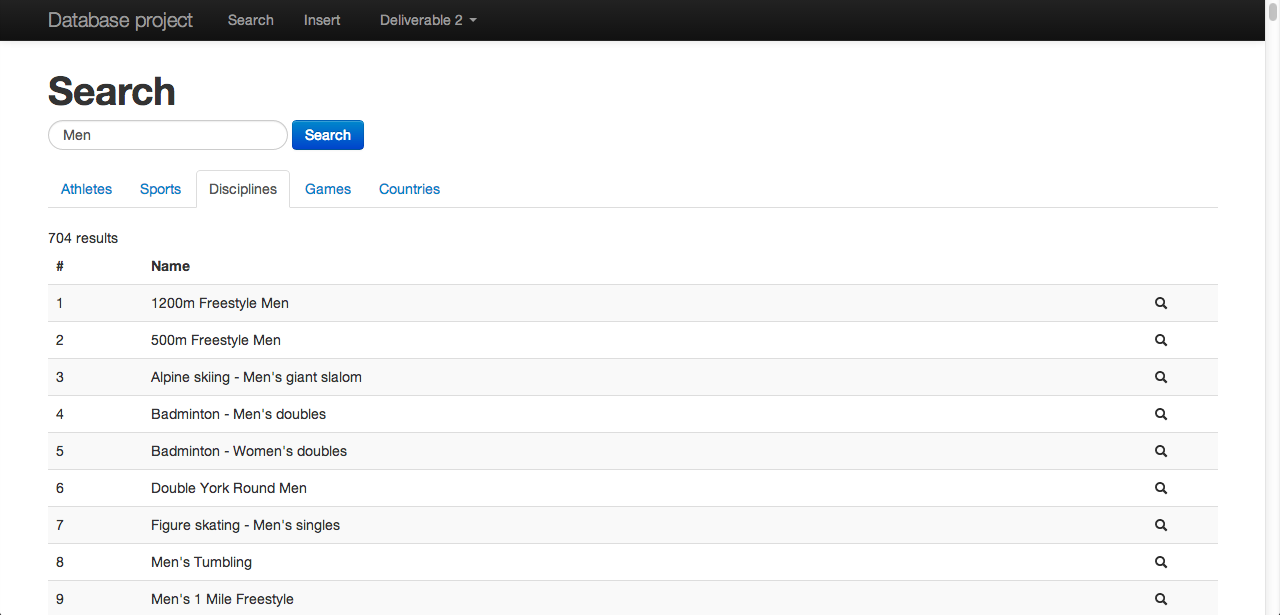
\includegraphics[height=210px]{images/capt2.png}
The search page
\end{center}

\begin{center}
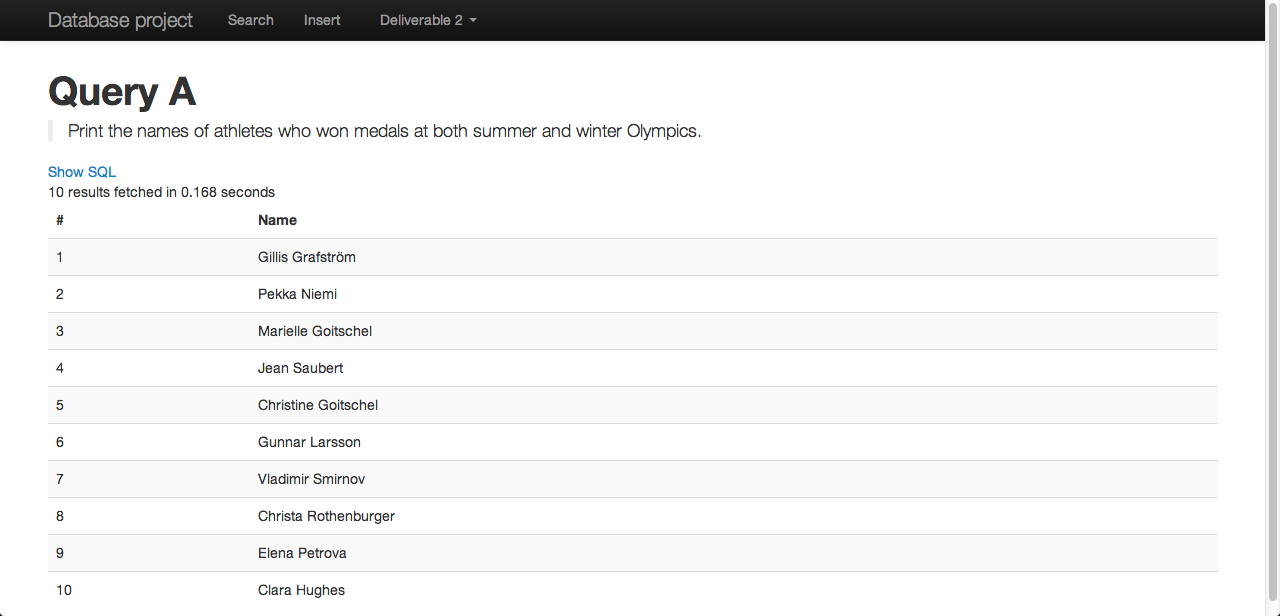
\includegraphics[height=210px]{images/capt3.png}
The result of one of the queries
\end{center}

\begin{center}
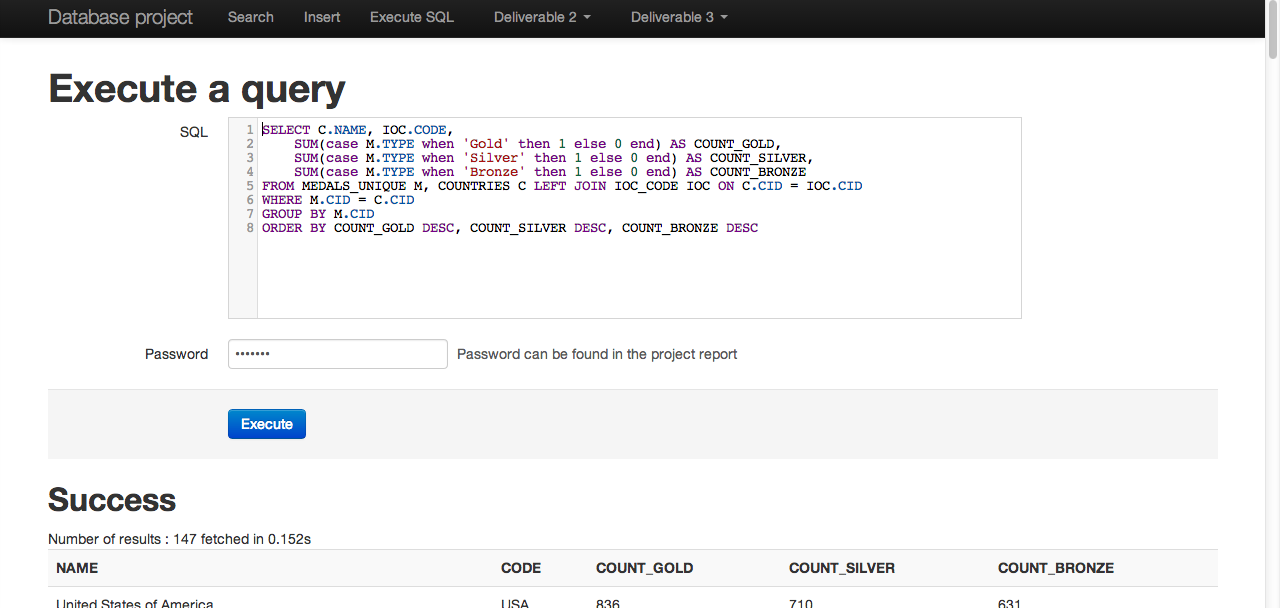
\includegraphics[height=210px]{images/capt4.png}
The interface to run queries
\end{center}













\part*{Queries}
\addcontentsline{toc}{section}{Queries}

\begin{enumerate}[A)]
	\item 
		Simple query using multiple ANDs
		\begin{lstlisting}
SELECT DISTINCT A.NAME 
FROM ATHLETES A, MEDALS M1, MEDALS M2, EVENTS E1, EVENTS E2, GAMES G1, GAMES G2
WHERE A.AID = M1.AID 
AND A.AID = M2.AID 
AND M1.MID <> M2.MID 
AND E1.EID = M1.EID 
AND E2.EID = M2.EID 
AND G1.GID = E1.GID 
AND G2.GID = E2.GID 
AND G1.TYPE <> G2.TYPE
		\end{lstlisting}
	\item 
		We have an outer-query which seeks gold medalist in sports that appear in the nested query, which computes all sports that have appeared only once
		\begin{lstlisting}
SELECT A.NAME AS ANAME, S.NAME AS SNAME
FROM SPORTS S, DISCIPLINES D, EVENTS E, ATHLETES A, MEDALS M
WHERE A.AID = M.AID 
AND M.TYPE = 'Gold' 
AND M.EID = E.EID 
AND E.DID = D.DID 
AND D.SID = S.SID 
AND S.SID IN (
	SELECT S2.SID
	FROM SPORTS S2, DISCIPLINES D2, EVENTS E2, GAMES G
	WHERE S2.SID = D2.SID 
	AND D2.DID = E2.DID 
	AND E2.GID = G.GID
	GROUP BY S2.SID
	HAVING Count(*)=1
)
ORDER BY A.NAME
		\end{lstlisting}
	\item 
		We retrieve the minimum year in which each country won its first medal using a subquery and then use a simple query to get the place hosting the corresponding games.
		\begin{lstlisting}
SELECT DISTINCT C.NAME, G.HOST_CITY
FROM COUNTRIES C, MEDALS M, EVENTS E, GAMES G, (
	SELECT C2.CID, MIN( G2.YEAR ) AS MIN_YEAR
	FROM COUNTRIES C2, MEDALS M2, EVENTS E2, GAMES G2
	WHERE C2.CID = M2.CID
	AND M2.EID = E2.EID
	AND E2.GID = G2.GID
	GROUP BY C2.CID
) TMP
WHERE C.CID = M.CID
AND M.EID = E.EID
AND E.GID = G.GID
AND C.CID = TMP.CID
AND G.YEAR = TMP.MIN_YEAR
ORDER BY C.NAME
		\end{lstlisting}
	\item 
		We unite (UNION) two same queries using "Summer" for one and "Winter" for the other and compute the number of medals for each country given the type (Summer or Winter), we then order them despondingly and limit the table to 1
		\begin{lstlisting}
(
	SELECT COUNT(M.CID) AS MAXIMUM, C.NAME, G.TYPE
	FROM COUNTRIES C, GAMES G, EVENTS E, MEDALS M
	WHERE C.CID = M.CID 
	AND M.EID = E.EID 
	AND E.GID = G.GID 
	AND G.TYPE = 'Summer'
	GROUP BY C.NAME 
	ORDER BY MAXIMUM DESC 
	LIMIT 1
) UNION (
	SELECT COUNT(M.CID) AS MAXIMUM, C.NAME, G.TYPE
	FROM COUNTRIES C, GAMES G, EVENTS E, MEDALS M
	WHERE C.CID = M.CID 
	AND M.EID = E.EID 
	AND E.GID = G.GID 
	AND G.TYPE = 'Winter'
	GROUP BY C.NAME 
	ORDER BY MAXIMUM DESC 
	LIMIT 1
)
		\end{lstlisting}
	\item 
		Simple GROUP BY + HAVING query
		\begin{lstlisting}
SELECT G.HOST_CITY
FROM GAMES G
GROUP BY G.HOST_CITY
HAVING COUNT(*) > 1
ORDER BY G.HOST_CITY
		\end{lstlisting}
	\item 
		We use two table of participants and two tables for countries and then just use ANDs to make find the athletes that competed for at least two countries
		\begin{lstlisting}
SELECT DISTINCT(A.NAME)
FROM ATHLETES A, PARTICIPANTS P1, PARTICIPANTS P2, COUNTRIES C1, COUNTRIES C2
WHERE A.AID = P1.AID 
AND A.AID = P2.AID 
AND P1.PID <> P2.PID 
AND P1.CID = C1.CID 
AND P2.CID = C2.CID 
AND C1.CID <> C2.CID
ORDER BY A.NAME
		\end{lstlisting}
	\item 
		The subquery computes the participants count for each country for a particular games. Then, for each game, the outer-query finds the countries having a participants count greater than all the results of the subquery.
		\begin{lstlisting}
SELECT G.YEAR, G.TYPE, C.NAME, COUNT(*) AS COUNT 
FROM COUNTRIES C, PARTICIPANTS P, GAMES G 
WHERE G.GID = P.GID AND C.CID=P.CID 
GROUP BY P.GID, P.CID 
HAVING COUNT(*) >= ALL (
	SELECT COUNT(*) 
	FROM PARTICIPANTS P2 
	WHERE P.GID=P2.GID 
	GROUP BY P2.GID, P2.CID
)
ORDER BY G.YEAR
		\end{lstlisting}
	\item 
		We simply take the COUNTRIES and use a nested query to delete all entries that do not appear in the MEDALS table
		\begin{lstlisting}
SELECT DISTINCT C.NAME
FROM COUNTRIES C
WHERE C.CID NOT IN (
	SELECT M.CID
	FROM MEDALS M
	WHERE M.CID IS NOT NULL
)
		\end{lstlisting}

	\item % I
		We simply use the sum function in our select clause incrementing the gold/silver/bronze count for each medal belonging to each country for some given games. We simply delete lines 7 and 8 when wanting to compute the table over all olympics.
		\begin{lstlisting}
SELECT C.NAME, IOC.CODE,
	SUM(case M.TYPE when 'Gold' then 1 else 0 end) AS COUNT_GOLD,
	SUM(case M.TYPE when 'Silver' then 1 else 0 end) AS COUNT_SILVER,
	SUM(case M.TYPE when 'Bronze' then 1 else 0 end) AS COUNT_BRONZE
FROM MEDALS_UNIQUE M, EVENTS E, COUNTRIES C LEFT JOIN IOC_CODE IOC ON C.CID = IOC.CID
WHERE M.CID = C.CID
AND M.EID = E.EID
AND E.GID = '3'
GROUP BY M.CID
ORDER BY COUNT_GOLD DESC, COUNT_SILVER DESC, COUNT_BRONZE DESC	

		\end{lstlisting}
	\item % J
		We use php to go through every SID in the SPORTS table and for each one simply grouped by the country and then ordered by their medal count descending and limited the result to 3. In the query below, the '?' would be replaced by each sport's SID.
		\begin{lstlisting}
SELECT C.NAME
FROM MEDALS_UNIQUE M, EVENTS E, DISCIPLINES D, COUNTRIES C
WHERE M.EID = E.EID
AND E.DID = D.DID
AND M.CID = C.CID
AND D.SID = ?
GROUP BY M.CID
ORDER BY COUNT(*) DESC
LIMIT 3	
		\end{lstlisting}
	\item % K
		The RANKING\_GLOBAL subquery computes the ranking in the medal tables of each game without restarting the position counter (the position in the medal table of the first games start at 1 but the first position of the next games starts at the last position of the previous one). The MIN\_RANKS subquery computes the minimal rank for each game such that we are now able to subtract the minimal rank to have each medal tables of GLOBAL\_RANKING starting at position 1; this is done in the RANKS\_PER\_GAMES subquery. The AVERAGE\_RANKS subquery computes the countries' average rank in the medal table of all games. Finally, we can compute the benefit for each country and each games by subtracting the rankings in AVERAGE\_RANK to the rankings RANKS\_PER\_GAMES and order the results by benefit.\\All this is done for individually for summer and winter. We unite their results with a UNION.
		\begin{lstlisting}
(
  SELECT G.YEAR, G.TYPE, C.NAME, RANKS_PER_GAMES.GID, AVERAGE_RANKS.RANK - RANKS_PER_GAMES.RANK AS BENEFIT FROM (
    SELECT RANKING_GLOBAL.GID, RANKING_GLOBAL.CID, RANKING_GLOBAL.RANK - MIN_RANKS.RANK + 1 AS RANK FROM (
      SELECT GID, MIN(RANK) AS RANK FROM (
        SELECT GID, CID, @rankA:=@rankA+1 AS RANK FROM (
          SELECT E.GID, M.CID,
            SUM(case M.TYPE when 'Gold' then 1 else 0 end) AS COUNT_GOLD,
            SUM(case M.TYPE when 'Silver' then 1 else 0 end) AS COUNT_SILVER,
            SUM(case M.TYPE when 'Bronze' then 1 else 0 end) AS COUNT_BRONZE
          FROM MEDALS_UNIQUE M, EVENTS E
          WHERE M.CID IS NOT NULL
          AND M.EID = E.EID
          GROUP BY M.CID, E.GID
          ORDER BY E.GID, COUNT_GOLD DESC, COUNT_SILVER DESC, COUNT_BRONZE DESC
        ) A, (SELECT @rankA:=0) INIT
      ) RANKING_GLOBAL
      GROUP BY RANKING_GLOBAL.GID
    ) MIN_RANKS, (
        SELECT GID, CID, @rankB:=@rankB+1 AS RANK FROM (
          SELECT E.GID, M.CID,
            SUM(case M.TYPE when 'Gold' then 1 else 0 end) AS COUNT_GOLD,
            SUM(case M.TYPE when 'Silver' then 1 else 0 end) AS COUNT_SILVER,
            SUM(case M.TYPE when 'Bronze' then 1 else 0 end) AS COUNT_BRONZE
          FROM MEDALS_UNIQUE M, EVENTS E
          WHERE M.CID IS NOT NULL
          AND M.EID = E.EID
          GROUP BY M.CID, E.GID
          ORDER BY E.GID, COUNT_GOLD DESC, COUNT_SILVER DESC, COUNT_BRONZE DESC
        ) B, (SELECT @rankB:=0) INIT
    ) RANKING_GLOBAL
    WHERE RANKING_GLOBAL.GID = MIN_RANKS.GID
  ) RANKS_PER_GAMES, (
    SELECT @rank1:=@rank1+1 AS RANK, MEDAL_TABLE.CID 
    FROM (SELECT M.CID,
        SUM(case M.TYPE when 'Gold' then 1 else 0 end) AS COUNT_GOLD,
        SUM(case M.TYPE when 'Silver' then 1 else 0 end) AS COUNT_SILVER,
        SUM(case M.TYPE when 'Bronze' then 1 else 0 end) AS COUNT_BRONZE
    FROM MEDALS_UNIQUE M
    GROUP BY M.CID
    ORDER BY COUNT_GOLD DESC, COUNT_SILVER DESC, COUNT_BRONZE DESC) MEDAL_TABLE, (SELECT @rank1:=0) INIT
  ) AVERAGE_RANKS, GAMES G, COUNTRIES C
  WHERE RANKS_PER_GAMES.GID = G.GID
  AND G.CID = C.CID
  AND AVERAGE_RANKS.CID = RANKS_PER_GAMES.CID
  AND G.CID = AVERAGE_RANKS.CID
  AND G.TYPE = 'Summer'
  ORDER BY BENEFIT DESC
  LIMIT 1
) UNION (
  SELECT G.YEAR, G.TYPE, C.NAME, RANKS_PER_GAMES.GID, AVERAGE_RANKS.RANK - RANKS_PER_GAMES.RANK AS BENEFIT FROM (
    SELECT RANKING_GLOBAL.GID, RANKING_GLOBAL.CID, RANKING_GLOBAL.RANK - MIN_RANKS.RANK + 1 AS RANK FROM (
      SELECT GID, MIN(RANK) AS RANK FROM (
        SELECT GID, CID, @rankC:=@rankC+1 AS RANK FROM (
          SELECT E.GID, M.CID,
            SUM(case M.TYPE when 'Gold' then 1 else 0 end) AS COUNT_GOLD,
            SUM(case M.TYPE when 'Silver' then 1 else 0 end) AS COUNT_SILVER,
            SUM(case M.TYPE when 'Bronze' then 1 else 0 end) AS COUNT_BRONZE
          FROM MEDALS_UNIQUE M, EVENTS E
          WHERE M.CID IS NOT NULL
          AND M.EID = E.EID
          GROUP BY M.CID, E.GID
          ORDER BY E.GID, COUNT_GOLD DESC, COUNT_SILVER DESC, COUNT_BRONZE DESC
        ) A, (SELECT @rankC:=0) INIT
      ) RANKING_GLOBAL
      GROUP BY RANKING_GLOBAL.GID
    ) MIN_RANKS, (
        SELECT GID, CID, @rankD:=@rankD+1 AS RANK FROM (
          SELECT E.GID, M.CID,
            SUM(case M.TYPE when 'Gold' then 1 else 0 end) AS COUNT_GOLD,
            SUM(case M.TYPE when 'Silver' then 1 else 0 end) AS COUNT_SILVER,
            SUM(case M.TYPE when 'Bronze' then 1 else 0 end) AS COUNT_BRONZE
          FROM MEDALS_UNIQUE M, EVENTS E
          WHERE M.CID IS NOT NULL
          AND M.EID = E.EID
          GROUP BY M.CID, E.GID
          ORDER BY E.GID, COUNT_GOLD DESC, COUNT_SILVER DESC, COUNT_BRONZE DESC
        ) B, (SELECT @rankD:=0) INIT
    ) RANKING_GLOBAL
    WHERE RANKING_GLOBAL.GID = MIN_RANKS.GID
  ) RANKS_PER_GAMES, (
    SELECT @rank2:=@rank2+1 AS RANK, MEDAL_TABLE.CID 
    FROM (SELECT M.CID,
        SUM(case M.TYPE when 'Gold' then 1 else 0 end) AS COUNT_GOLD,
        SUM(case M.TYPE when 'Silver' then 1 else 0 end) AS COUNT_SILVER,
        SUM(case M.TYPE when 'Bronze' then 1 else 0 end) AS COUNT_BRONZE
    FROM MEDALS_UNIQUE M
    GROUP BY M.CID
    ORDER BY COUNT_GOLD DESC, COUNT_SILVER DESC, COUNT_BRONZE DESC) MEDAL_TABLE, (SELECT @rank2:=0) INIT
  ) AVERAGE_RANKS, GAMES G, COUNTRIES C
  WHERE RANKS_PER_GAMES.GID = G.GID
  AND G.CID = C.CID
  AND AVERAGE_RANKS.CID = RANKS_PER_GAMES.CID
  AND G.CID = AVERAGE_RANKS.CID
  AND G.TYPE = 'Winter'
  ORDER BY BENEFIT DESC
  LIMIT 1
)
		\end{lstlisting}
	\item % L
		Here we simply count the number of medalists per country (that is counting the multiple medals when a team has won) and divide it by the number of unique medals per country (that is only counting one medal when a team has one) therefore giving us the average number of athletes per medal per country.  
		\begin{lstlisting}
SELECT C.NAME, MEDALISTS_COUNT.COUNT / MEDALS_COUNT.COUNT AS MEDALISTS_PER_MEDAL 
FROM COUNTRIES C, (
	SELECT M.CID, COUNT(*) AS COUNT
	FROM MEDALS M
	GROUP BY M.CID
) MEDALISTS_COUNT,
(
	SELECT MU.CID, COUNT(*) AS COUNT
	FROM MEDALS_UNIQUE MU
	GROUP BY MU.CID
) MEDALS_COUNT
WHERE MEDALISTS_COUNT.CID = MEDALS_COUNT.CID
AND MEDALISTS_COUNT.CID = C.CID
ORDER BY MEDALISTS_PER_MEDAL DESC
LIMIT 10
		\end{lstlisting}
	\item % M
		For this query we just computed all the athletes that whale at least two medals having a different countries.
		\begin{lstlisting}
SELECT DISTINCT A.NAME
FROM ATHLETES A, MEDALS M1, MEDALS M2
WHERE M1.CID <> M2.CID
AND M1.AID = M2.AID
AND M1.AID = A.AID
ORDER BY A.NAME	
		\end{lstlisting}
	\item % N
		For this one we used a little trick using a case in a case. We associate gold to 1, silver to 2 and bronze to 3 and take the minimum so that is a country has one multiple medals at their first olympics we will only consider the shinier. Whoever we are now left with 1,2 or 3 therefore, there is a second case reverting 1 to gold, 2 to silver and 3 to bronze. For the rest we simply look for the first olympics where each country won it's first medal.
		\begin{lstlisting}
SELECT C.NAME, 
case MIN(case M.TYPE 
		WHEN 'Gold' THEN 1 
		WHEN 'Silver' THEN 2 
		WHEN 'Bronze' THEN 3 
		end) 
	WHEN 1 THEN 'Gold' 
	WHEN 2 THEN 'Silver' 
	WHEN 3 THEN 'Bronze' 
end AS TYPE, G.YEAR
FROM COUNTRIES C, MEDALS M, EVENTS E, GAMES G
WHERE M.CID = C.CID
AND M.EID = E.EID
AND E.GID = G.GID
GROUP BY C.NAME
HAVING G.YEAR = MIN(G.YEAR)
ORDER BY C.NAME	
		\end{lstlisting}
	\item % O
		Here we look for a country that has won medals in to different events but for the same discipline and then compute the biggest time lapse between those to medals.
		\begin{lstlisting}
SELECT D.NAME AS DNAME, C.NAME AS CNAME, MAX(G2.YEAR-G1.YEAR) AS TIME
FROM COUNTRIES C, EVENTS E1, EVENTS E2, GAMES G1, GAMES G2, DISCIPLINES D, MEDALS M1, MEDALS M2
WHERE M1.EID = E1.EID
AND M2.EID = E2.EID
AND E1.EID <> E2.EID
AND M1.CID = M2.CID
AND M1.CID = C.CID
AND E1.DID = E2.DID
AND E1.DID = D.DID
AND D.DID = ?
AND E1.GID = G1.GID
AND E2.GID = G2.GID
AND G1.YEAR < G2.YEAR
GROUP BY C.NAME
ORDER BY TIME DESC LIMIT 1
		\end{lstlisting}
	\item % P
		For this query for each event we counted the number of distinct countries that won a medal and then only considered the events were that had a count equal to 1.
		\begin{lstlisting}
SELECT D.NAME, G.TYPE, G.YEAR
FROM (
	SELECT E.EID, COUNT(DISTINCT M.CID) AS NBR
	FROM EVENTS E, MEDALS M
	WHERE M.EID = E.EID
	GROUP BY E.EID
) COUNTRIES_COUNTS, 
EVENTS E, DISCIPLINES D, GAMES G
WHERE E.EID = COUNTRIES_COUNTS.EID
AND COUNTRIES_COUNTS.NBR = 1
AND E.DID = D.DID
AND E.GID = G.GID
ORDER BY G.YEAR	
		\end{lstlisting}
	\item % Q
		We used again php to go through our games and for each one we counted the number of medals for each countries and foreach divided it by the total number of medals for those games. In the code below the '?' is replaced with each GID.
		\begin{lstlisting}
SELECT C.NAME,
ROUND(COUNT(*) / (
	SELECT COUNT(*) 
	FROM MEDALS M, EVENTS E 
	WHERE E.EID=M.EID 
	AND E.GID=?
) * 100, 2) AS PERCENT
FROM EVENTS E, MEDALS M, COUNTRIES C
WHERE E.GID=? 
AND E.EID=M.EID 
AND C.CID=M.CID
GROUP BY M.CID
ORDER BY PERCENT DESC
LIMIT 1	
		\end{lstlisting}
	\item % R
		For each event and each medal type, we compute a "shared coefficient" which is 2 if the medal is shared and 1 otherwise. Then we simply sum the points associated with each medal and divide it by the "shared coeffficient" such that shared medals are worth half the points. 
		\begin{lstlisting}
SELECT C.NAME, SUM(
    case M.TYPE 
        when 'Gold' then 3/SHARED_COEFF.COEFF
        when 'Silver' then 2/SHARED_COEFF.COEFF
        when 'Bronze' then 1/SHARED_COEFF.COEFF
    end
) AS SCORE
FROM MEDALS M, COUNTRIES C, EVENTS E, DISCIPLINES D, (
    SELECT M.EID, M.TYPE, (
        case COUNT(M.MID) 
            when 1 then 1 
            else 2 
        end
    ) AS COEFF
    FROM MEDALS M
    GROUP BY M.EID, M.TYPE
) AS SHARED_COEFF
WHERE M.CID = C.CID
AND M.TID IS NULL
AND M.EID = E.EID
AND E.DID = D.DID
AND M.EID = SHARED_COEFF.EID
AND M.TYPE = SHARED_COEFF.TYPE
AND D.SID = ?
GROUP BY C.CID
ORDER BY SCORE DESC
LIMIT 10
		\end{lstlisting}
	\item % S
		For this one we simply compute all athletes for which there exists at least one individual medal (TID is NULL) and one team medal (TID isn't NULL).
		\begin{lstlisting}
SELECT DISTINCT A.NAME
FROM ATHLETES A, MEDALS M1, MEDALS M2
WHERE A.AID = M1.AID
AND A.AID = M2.AID
AND M1.TID IS NOT NULL
AND M2.TID IS NULL
ORDER BY A.NAME
		\end{lstlisting}
	\item % T
		Here we first look for the athletes that have a gold medal in a team sport, then that the said athlete also won an individual medal but that there does not exist a medal such that it belongs to the said athlete, is of type Gold and is individual (TID is NULL). Therefore meaning that his individual medals could only be silver or bronze.
		\begin{lstlisting}
SELECT DISTINCT A.NAME
FROM ATHLETES A, MEDALS M1, MEDALS M2
WHERE A.AID = M1.AID
AND M1.TID IS NOT NULL
AND M1.TYPE = 'Gold'
AND A.AID = M2.AID
AND M2.TID IS NULL
AND NOT EXISTS ( SELECT M3.MID 
	FROM MEDALS M3 
	WHERE M3.AID = A.AID 
	AND M3.TID IS NULL 
	AND M3.TYPE = 'Gold')
ORDER BY A.NAME
		\end{lstlisting}
	\item % U
		Here we are only looking for gold medals that have been won in consecutive games. To do so we first check that a gold medal was won for the same discipline in the most recent game where that discipline appeared. To do so we take the biggest year that is lower than year of the game of the first medal. We know only have to check is there wasn't another game in between where the discipline didn't appear. (The computation goes quite faster if we don't care if onlympics occurred in-between without the said discipline)
		\begin{lstlisting}
SELECT DISTINCT D.NAME, C.NAME AS CNAME, G.TYPE, G.YEAR AS YEAR1, G2.YEAR AS YEAR2, M.TYPE AS MTYPE
FROM MEDALS M, EVENTS E, GAMES G, DISCIPLINES D, COUNTRIES C, GAMES G2, EVENTS E2, MEDALS M2
WHERE M.TYPE = 'Gold'
AND M.EID = E.EID
AND G.GID = E.GID
AND C.CID = M.CID
AND D.DID = E.DID
AND M2.TYPE = 'Gold'
AND M2.EID = ( 
	SELECT E1.EID
	FROM GAMES G1, 
	EVENTS E1
	WHERE G1.YEAR < G.YEAR
	AND G1.TYPE = G.TYPE
	AND E1.GID = G1.GID
	AND E1.DID = E.DID
	AND NOT EXISTS (
		SELECT * 
		FROM GAMES G2
		WHERE G2.YEAR < G.YEAR
		AND G2.YEAR > G1.YEAR
		AND G2.TYPE = G.TYPE
	)
	ORDER BY G1.YEAR DESC 
	LIMIT 1 
)
AND E2.EID = M2.EID
AND G2.GID = E2.GID
AND M.CID = M2.CID	
		\end{lstlisting}
	\item % V
		We determine in a subquery in our FROM clause the events to consider, that is the events that are appearing for the first time at the olympics. We then simply do the same sum as for query I) to sum the gold, silver and bronze medals.
		\begin{lstlisting}
SELECT C.NAME, IOC.CODE,
	SUM(case M.TYPE when 'Gold' then 1 else 0 end) AS COUNT_GOLD,
	SUM(case M.TYPE when 'Silver' then 1 else 0 end) AS COUNT_SILVER,
	SUM(case M.TYPE when 'Bronze' then 1 else 0 end) AS COUNT_BRONZE
FROM MEDALS_UNIQUE M, COUNTRIES C LEFT JOIN IOC_CODE IOC ON C.CID = IOC.CID, (
	SELECT E.EID
	FROM EVENTS E, GAMES G, (
		SELECT E.DID, MIN(G.YEAR) AS YEAR
		FROM EVENTS E, GAMES G
		WHERE E.GID = G.GID
		GROUP BY E.DID
	) FIRST_APPEARANCE
	WHERE E.GID = G.GID
	AND E.DID = FIRST_APPEARANCE.DID
	AND G.YEAR = FIRST_APPEARANCE.YEAR
	ORDER BY E.EID  
) EVENTS_TO_CONSIDER
WHERE M.CID = C.CID
AND M.EID = EVENTS_TO_CONSIDER.EID
GROUP BY M.CID
ORDER BY COUNT_GOLD DESC, COUNT_SILVER DESC, COUNT_BRONZE DESC
LIMIT 10
		\end{lstlisting}
\end{enumerate}

\end{document}